\documentclass{article}
\usepackage[utf8]{inputenc}
\usepackage{graphicx}
\author{Felix Bello, Gilles Brunner}
\title{Arbeitsauftrag 2}
\begin{document}
	\maketitle
	\section{Einführung}
Nachstehend wird beschrieben, wie wir für eine Wordpress-Installation im Rahmen des Moduls IKS vorgehen. Da wir die Aufgabe auf unserem Debian-Server lösen, gibt es einige Unterschiede bei gewissen Namen: Apache ist nicht unter httpd zu finden, sondern Apache2 und Benutzer und die Gruppe für unseren Webpfad ist www-data (das nur als Info, damit ist kein Durcheinander gibt bei der Aufführung unsere Pfade und 	Benutzerberechtigungen.)
	\section{LAMP}
	\textit{lucy:/home/gilles\# screen -S newScreen}
	\newline
	\textit{lucy:/home/gilles\# apt-get install mariadb-client-10.0 mariadb-server-10.0 apache2 apache2-doc php5 php5-mysql libapache 2-mod-php5}
	\newline
	
	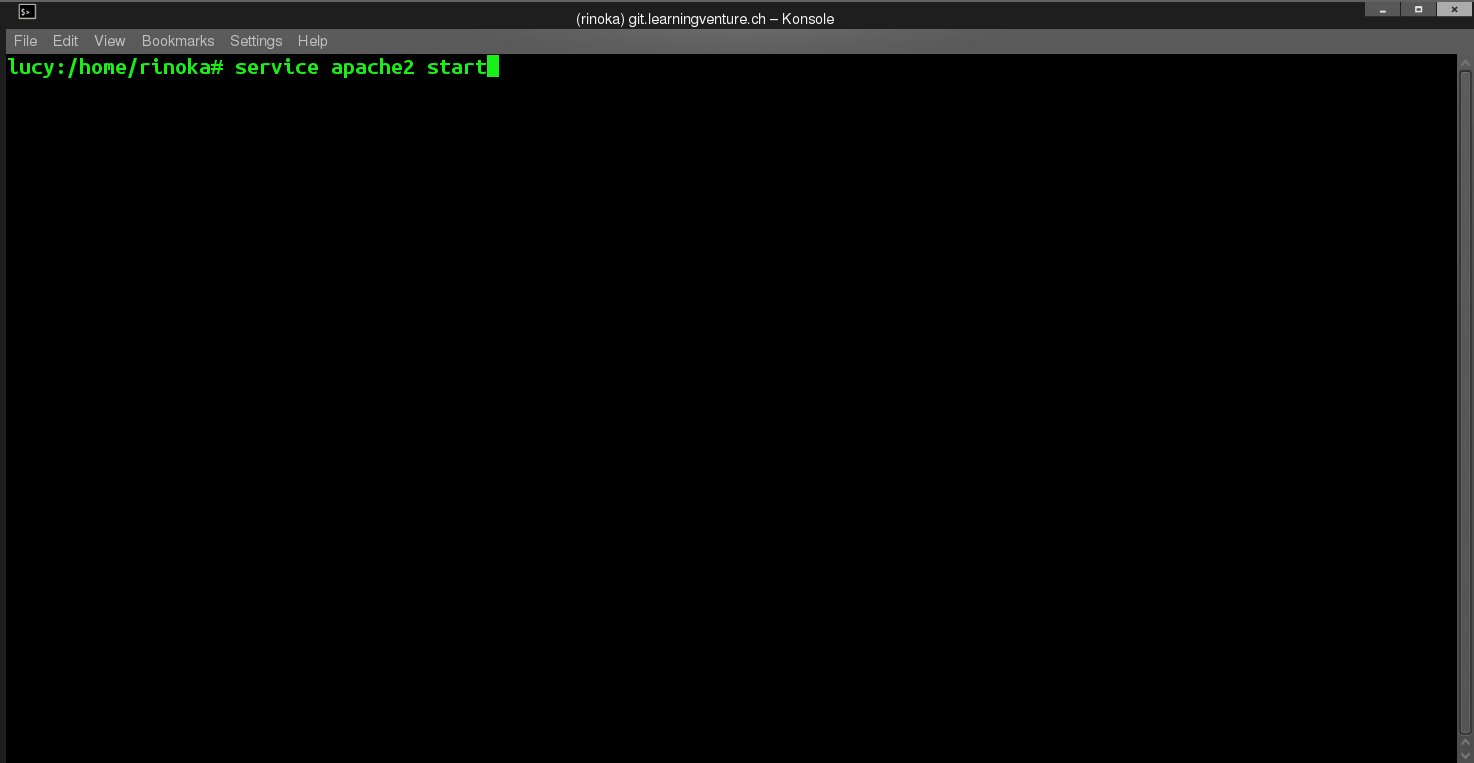
\includegraphics[width=13cm]{../Pics/start_apache}
	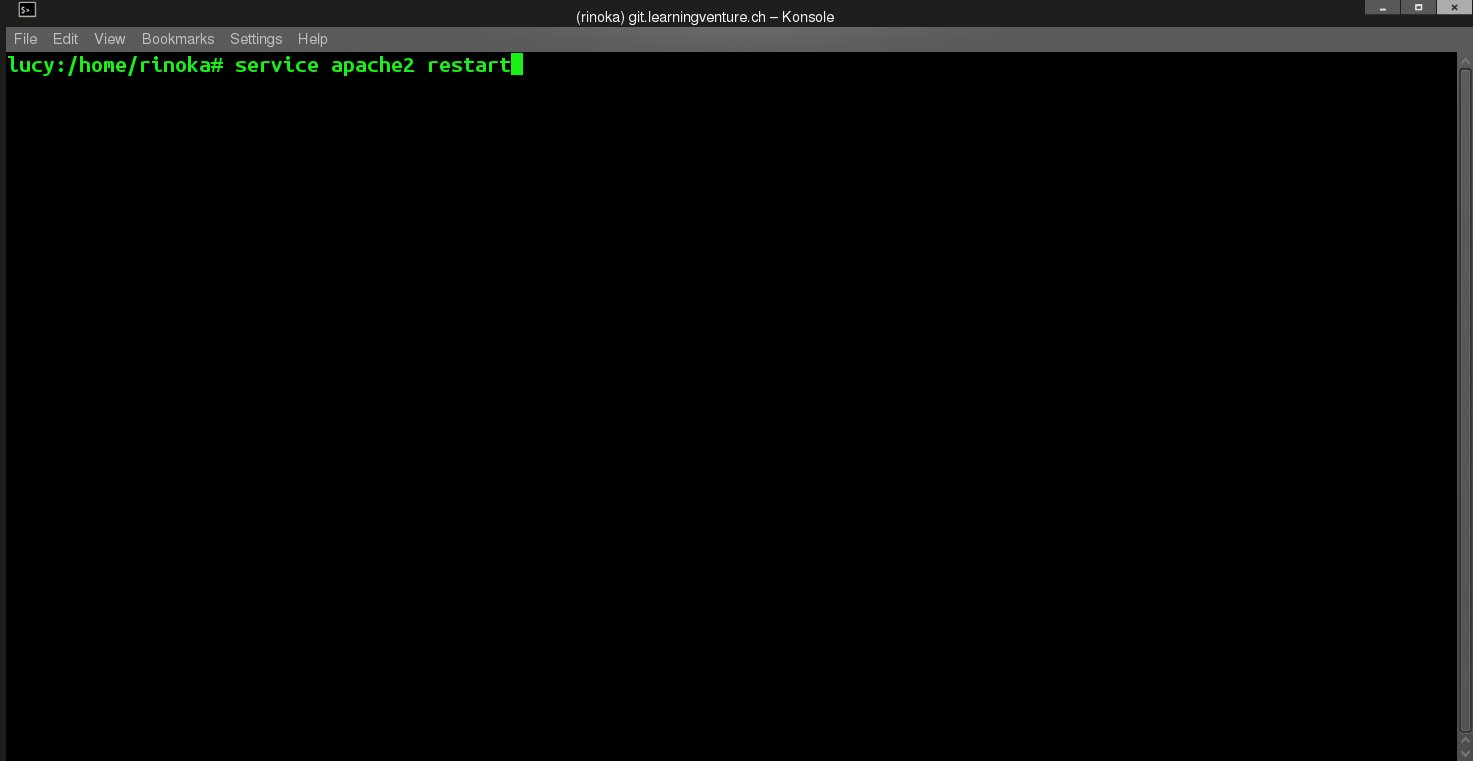
\includegraphics[width=13cm]{../Pics/apach2restart}
	\subsection{Linux}
	\subsection{Apache}
	Gemäss der im Auftrag erfordlichen Konfigurationsdateien muss die Wordpress-Installation auf dem Server unter folgendem Dateipfad installiert werden: /var/www/html/wordpress.
	Allerdings soll Wordpress auf IP-Adresse/blog aufgerufen werden. Dazu muss der VirtualHost in /etc/apache2/sites-available/ angepasst werden.
	\subsection{VirtualHost}
	Die Dokumentation, die wir uns für die erforderliche VirtualHost-Konfiguration angeschaut haben, befindet sich hier: https://httpd.apache.org/docs/2.2/mod/mod_alias.html\#alias
	Die Idee ist folgende:
	The directives contained in this module allow for manipulation and control of URLs as requests arrive at the server. The Alias and ScriptAlias directives are used to map between URLs and filesystem paths.
	Das heisst, dass man mit einer bestimmten URL (in unserem Falle IP-adresse/blog) auf einen bestimmten Pfad auf dem Server selbst zugreifen kann (in unserem Falle /var/www/html/wordpress). Dazu muss die VirtualHost- Konfigurationsdatei in /etc/apache2/sites-available/wordpress.conf entsprechend angepasst werden:
	\subsection{MariaDB}
	Wir haben uns wie bereits erwähnt für \textit{\textbf{MariaDB}}  als Datenbank entschieden, um diese zu Konfigurieren wird automatisch vom installer, den wir bereits ausgeführt haben mit \textit{\textbf{lucy:/home/gilles\# apt-get install mariadb-client-10.0 mariadb-server-10.0 apache2 apache2-doc php5 php5-mysql libapache 2-mod-php5}} die passwortabfrage angezeigt.
	\newline
	\newline
	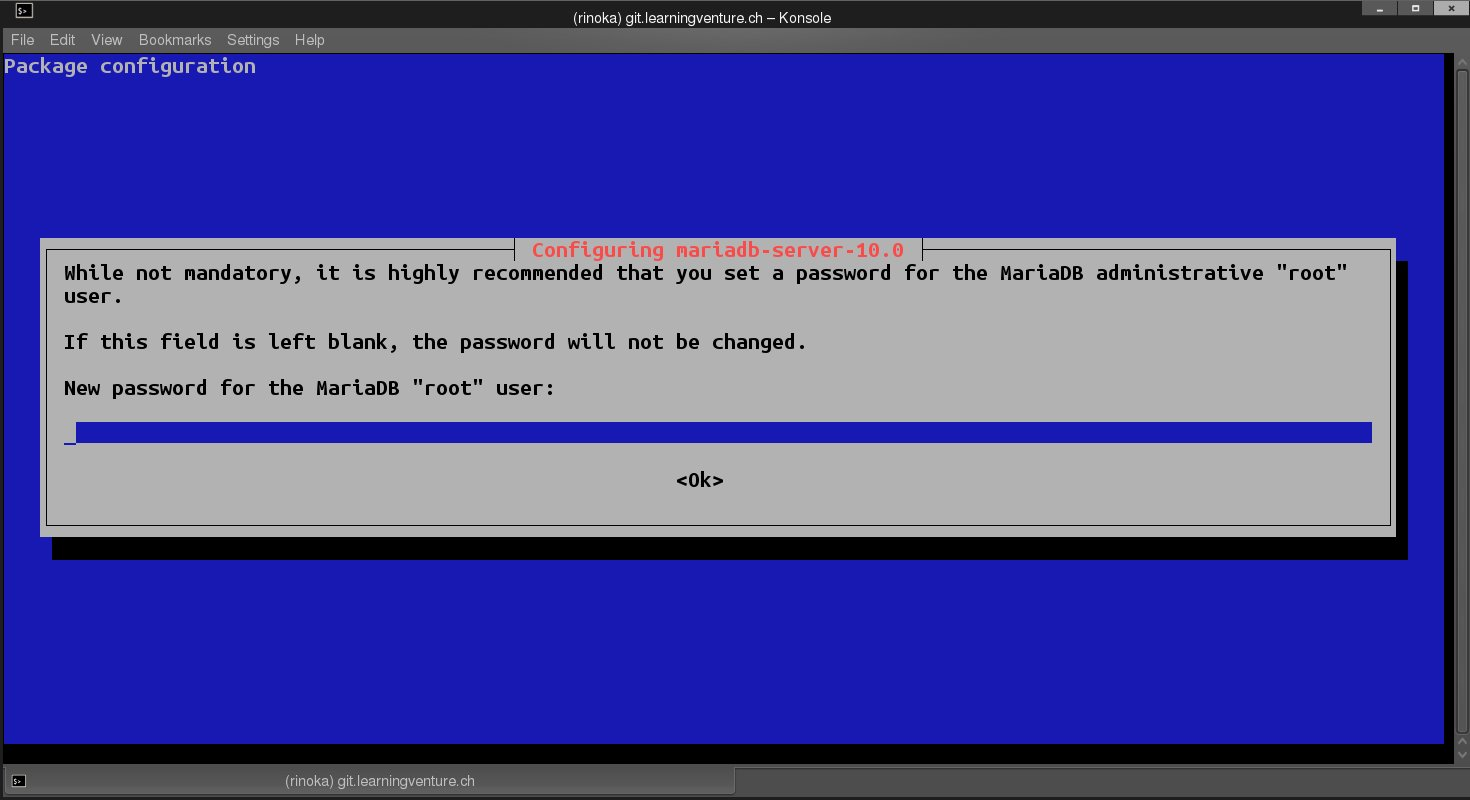
\includegraphics[width=13cm]{../Pics/3-lamp-stack-mariadb}
	\newline
	\newline
	Hier folgt natürlich nun die Datenbank erstellung, wie folgt:
	\subsection{PHP}
	\section{WordPress}
	\section{OwnCloud}
\end{document}